\section{oosalizer/preserve.c-Dateireferenz}
\label{preserve_8c}\index{oosalizer/preserve.c@{oosalizer/preserve.c}}
{\tt \#include $<$time.h$>$}\par
{\tt \#include $<$stdio.h$>$}\par
{\tt \#include $<$stdlib.h$>$}\par
{\tt \#include $<$string.h$>$}\par
{\tt \#include $<$unistd.h$>$}\par
{\tt \#include $<$ctype.h$>$}\par
{\tt \#include $<$sys/utsname.h$>$}\par
{\tt \#include $<$sys/times.h$>$}\par
{\tt \#include $<$sys/types.h$>$}\par
{\tt \#include \char`\"{}webalizer.h\char`\"{}}\par
{\tt \#include \char`\"{}lang.h\char`\"{}}\par
{\tt \#include \char`\"{}hashtab.h\char`\"{}}\par
{\tt \#include \char`\"{}parser.h\char`\"{}}\par
{\tt \#include \char`\"{}preserve.h\char`\"{}}\par


Include-Abh\"{a}ngigkeitsdiagramm f\"{u}r preserve.c:\begin{figure}[H]
\begin{center}
\leavevmode
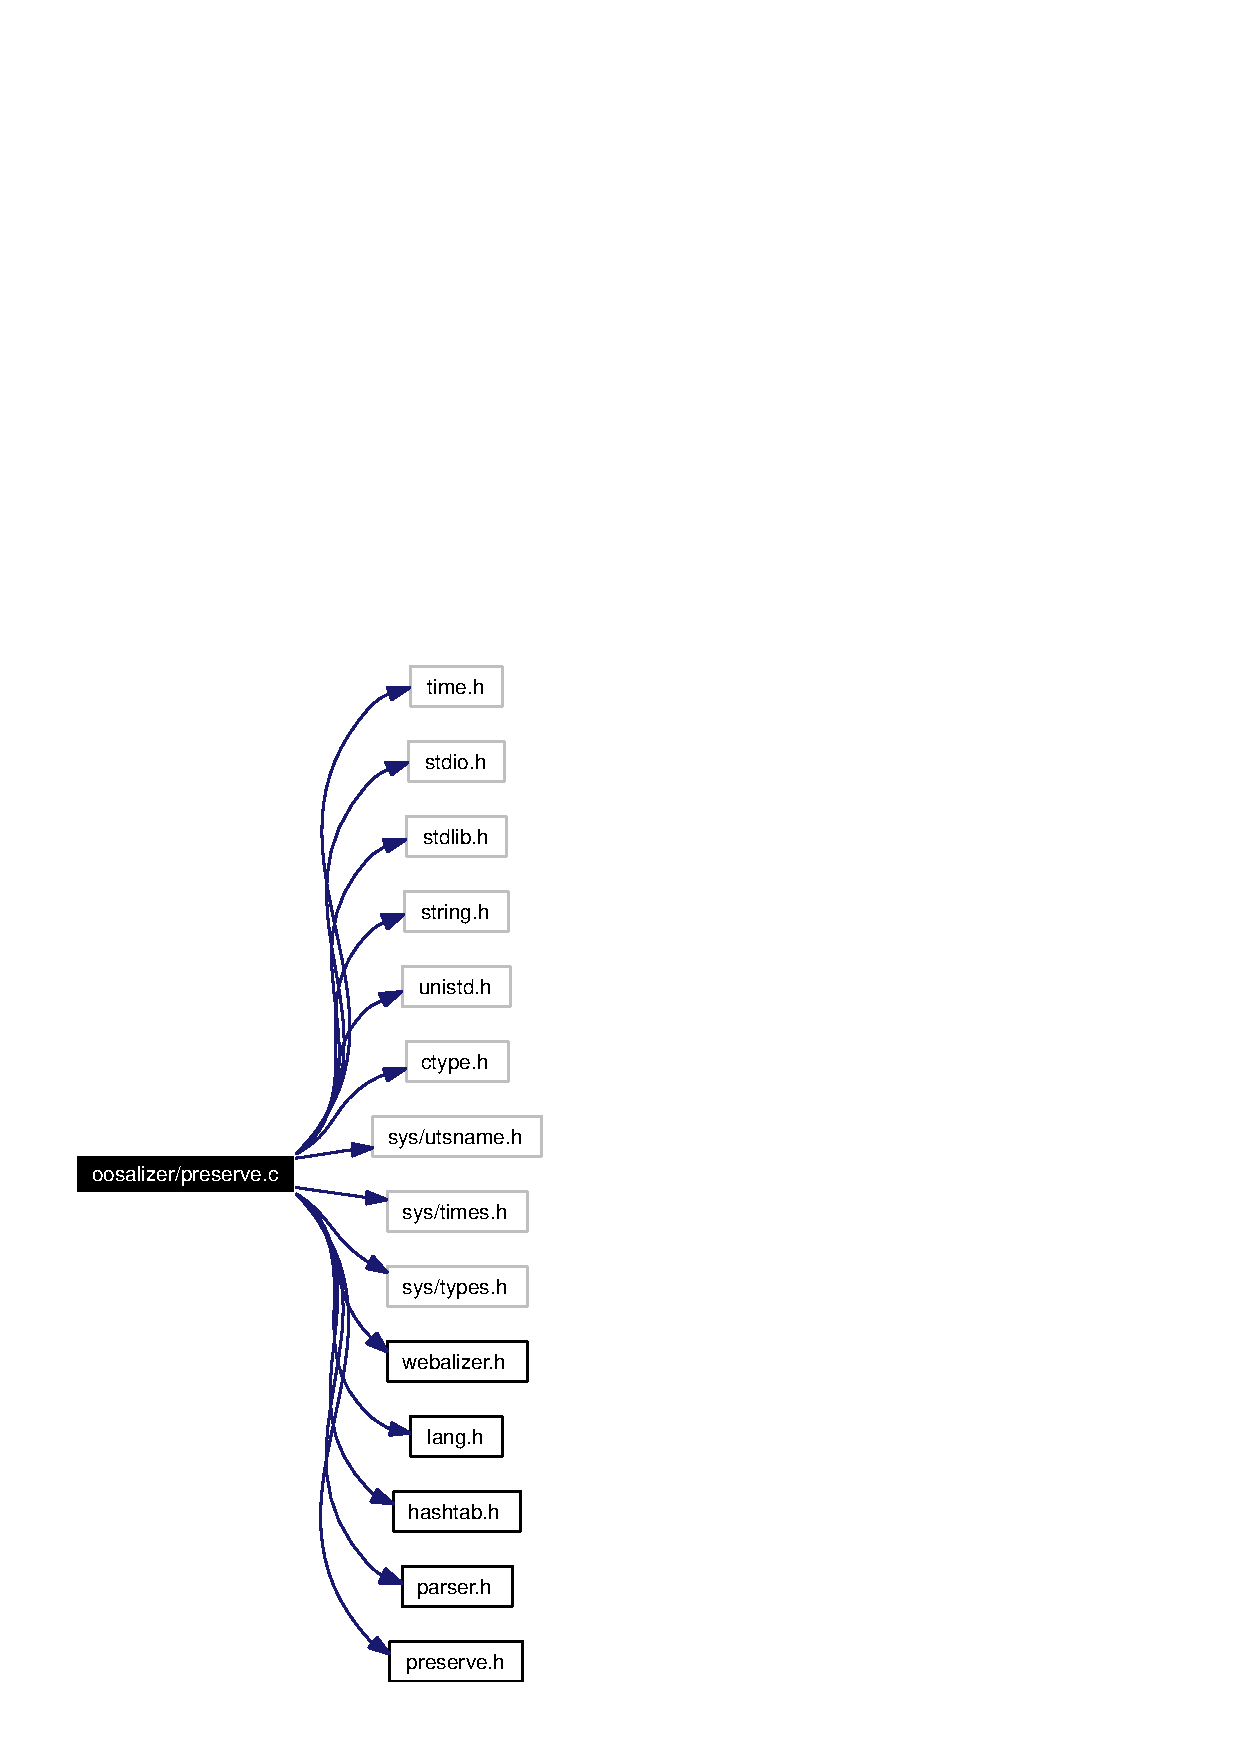
\includegraphics[width=130pt]{preserve_8c__incl}
\end{center}
\end{figure}
\subsection*{Makrodefinitionen}
\begin{CompactItemize}
\item 
\#define {\bf CLK\_\-TCK}~\_\-SC\_\-CLK\_\-TCK
\end{CompactItemize}
\subsection*{Funktionen}
\begin{CompactItemize}
\item 
void {\bf get\_\-history} ()
\item 
void {\bf put\_\-history} ()
\item 
int {\bf save\_\-state} ()
\item 
int {\bf restore\_\-state} ()
\end{CompactItemize}
\subsection*{Variablen}
\begin{CompactItemize}
\item 
int {\bf hist\_\-month} [12]
\item 
int {\bf hist\_\-year} [12]
\item 
u\_\-long {\bf hist\_\-hit} [12]
\item 
u\_\-long {\bf hist\_\-files} [12]
\item 
u\_\-long {\bf hist\_\-site} [12]
\item 
double {\bf hist\_\-xfer} [12]
\item 
u\_\-long {\bf hist\_\-page} [12]
\item 
u\_\-long {\bf hist\_\-visit} [12]
\item 
int {\bf hist\_\-fday} [12]
\item 
int {\bf hist\_\-lday} [12]
\end{CompactItemize}


\subsection{Makro-Dokumentation}
\index{preserve.c@{preserve.c}!CLK_TCK@{CLK\_\-TCK}}
\index{CLK_TCK@{CLK\_\-TCK}!preserve.c@{preserve.c}}
\subsubsection{\setlength{\rightskip}{0pt plus 5cm}\#define CLK\_\-TCK~\_\-SC\_\-CLK\_\-TCK}\label{preserve_8c_03df76d1f70664d745ca8de2864e39b3}




Definiert in Zeile 59 der Datei preserve.c.

\subsection{Dokumentation der Funktionen}
\index{preserve.c@{preserve.c}!get_history@{get\_\-history}}
\index{get_history@{get\_\-history}!preserve.c@{preserve.c}}
\subsubsection{\setlength{\rightskip}{0pt plus 5cm}void get\_\-history ()}\label{preserve_8c_d7ce84df67f8fe6fb2ae68f70445e3ff}




Definiert in Zeile 83 der Datei preserve.c.

Benutzt buffer, BUFSIZE, hist\_\-fday, hist\_\-files, hist\_\-hit, hist\_\-lday, hist\_\-month, hist\_\-page, hist\_\-site, hist\_\-visit, hist\_\-xfer und hist\_\-year.\index{preserve.c@{preserve.c}!put_history@{put\_\-history}}
\index{put_history@{put\_\-history}!preserve.c@{preserve.c}}
\subsubsection{\setlength{\rightskip}{0pt plus 5cm}void put\_\-history ()}\label{preserve_8c_0725425e14f501da1e2fc612d7854c01}




Definiert in Zeile 140 der Datei preserve.c.

Benutzt hist\_\-fday, hist\_\-files, hist\_\-fname, hist\_\-hit, hist\_\-lday, hist\_\-month, hist\_\-page, hist\_\-site, hist\_\-visit, hist\_\-xfer, hist\_\-year, msg\_\-put\_\-hist und verbose.\index{preserve.c@{preserve.c}!restore_state@{restore\_\-state}}
\index{restore_state@{restore\_\-state}!preserve.c@{preserve.c}}
\subsubsection{\setlength{\rightskip}{0pt plus 5cm}int restore\_\-state ()}\label{preserve_8c_87684b62a3f6bfdc76f25d5fb679c901}




Definiert in Zeile 405 der Datei preserve.c.

Benutzt BUFSIZE, cur\_\-day, cur\_\-hour, cur\_\-min, cur\_\-month, cur\_\-sec, cur\_\-tstamp, cur\_\-year, epoch, jdate(), msg\_\-get\_\-data, msg\_\-no\_\-data, state\_\-fname, t\_\-agent, t\_\-file, t\_\-hit, t\_\-page, t\_\-ref, t\_\-site, t\_\-url, t\_\-user, t\_\-visit, t\_\-xfer, tmp\_\-buf, ul\_\-bogus, verbose und version.\index{preserve.c@{preserve.c}!save_state@{save\_\-state}}
\index{save_state@{save\_\-state}!preserve.c@{preserve.c}}
\subsubsection{\setlength{\rightskip}{0pt plus 5cm}int save\_\-state ()}\label{preserve_8c_30d384683c4584a041792cf314051fa3}




Definiert in Zeile 178 der Datei preserve.c.

Benutzt buffer, BUFSIZE, cur\_\-day, cur\_\-hour, cur\_\-min, cur\_\-month, cur\_\-sec, cur\_\-year, dt\_\-site, editlvl, f\_\-day, ht\_\-hit, l\_\-day, mh\_\-hit, msg\_\-put\_\-data, state\_\-fname, t\_\-agent, t\_\-file, t\_\-hit, t\_\-page, t\_\-ref, t\_\-site, t\_\-url, t\_\-user, t\_\-visit, t\_\-xfer, tm\_\-file, tm\_\-hit, tm\_\-page, tm\_\-site, tm\_\-visit, tm\_\-xfer, verbose und version.

\subsection{Variablen-Dokumentation}
\index{preserve.c@{preserve.c}!hist_fday@{hist\_\-fday}}
\index{hist_fday@{hist\_\-fday}!preserve.c@{preserve.c}}
\subsubsection{\setlength{\rightskip}{0pt plus 5cm}int {\bf hist\_\-fday}[12]}\label{preserve_8c_aa2fe5b00c099187be9c1aace6552a9c}




Definiert in Zeile 77 der Datei preserve.c.

Wird benutzt von get\_\-history(), put\_\-history() und write\_\-month\_\-html().\index{preserve.c@{preserve.c}!hist_files@{hist\_\-files}}
\index{hist_files@{hist\_\-files}!preserve.c@{preserve.c}}
\subsubsection{\setlength{\rightskip}{0pt plus 5cm}u\_\-long {\bf hist\_\-files}[12]}\label{preserve_8c_5fce0b39aa3228d6b471e9294f1fed9d}




Definiert in Zeile 71 der Datei preserve.c.

Wird benutzt von get\_\-history(), put\_\-history() und write\_\-month\_\-html().\index{preserve.c@{preserve.c}!hist_hit@{hist\_\-hit}}
\index{hist_hit@{hist\_\-hit}!preserve.c@{preserve.c}}
\subsubsection{\setlength{\rightskip}{0pt plus 5cm}u\_\-long {\bf hist\_\-hit}[12]}\label{preserve_8c_71b324074ec02105c3730f77c0ab3e50}




Definiert in Zeile 70 der Datei preserve.c.

Wird benutzt von get\_\-history(), put\_\-history() und write\_\-month\_\-html().\index{preserve.c@{preserve.c}!hist_lday@{hist\_\-lday}}
\index{hist_lday@{hist\_\-lday}!preserve.c@{preserve.c}}
\subsubsection{\setlength{\rightskip}{0pt plus 5cm}int {\bf hist\_\-lday}[12]}\label{preserve_8c_c1366de31d95191e4f8fe0894dabb4e2}




Definiert in Zeile 77 der Datei preserve.c.

Wird benutzt von daily\_\-total\_\-table(), get\_\-history(), put\_\-history() und write\_\-month\_\-html().\index{preserve.c@{preserve.c}!hist_month@{hist\_\-month}}
\index{hist_month@{hist\_\-month}!preserve.c@{preserve.c}}
\subsubsection{\setlength{\rightskip}{0pt plus 5cm}int {\bf hist\_\-month}[12]}\label{preserve_8c_8dbdfde33bef98c2e3a8d2b8fab9143d}




Definiert in Zeile 69 der Datei preserve.c.

Wird benutzt von get\_\-history(), put\_\-history(), write\_\-main\_\-index() und write\_\-month\_\-html().\index{preserve.c@{preserve.c}!hist_page@{hist\_\-page}}
\index{hist_page@{hist\_\-page}!preserve.c@{preserve.c}}
\subsubsection{\setlength{\rightskip}{0pt plus 5cm}u\_\-long {\bf hist\_\-page}[12]}\label{preserve_8c_6885f98057e49be4b1a58cc1fea67b11}




Definiert in Zeile 74 der Datei preserve.c.

Wird benutzt von get\_\-history(), put\_\-history() und write\_\-month\_\-html().\index{preserve.c@{preserve.c}!hist_site@{hist\_\-site}}
\index{hist_site@{hist\_\-site}!preserve.c@{preserve.c}}
\subsubsection{\setlength{\rightskip}{0pt plus 5cm}u\_\-long {\bf hist\_\-site}[12]}\label{preserve_8c_95f554bfcd0bb37a1e90b29db92d2ffa}




Definiert in Zeile 72 der Datei preserve.c.

Wird benutzt von get\_\-history(), put\_\-history() und write\_\-month\_\-html().\index{preserve.c@{preserve.c}!hist_visit@{hist\_\-visit}}
\index{hist_visit@{hist\_\-visit}!preserve.c@{preserve.c}}
\subsubsection{\setlength{\rightskip}{0pt plus 5cm}u\_\-long {\bf hist\_\-visit}[12]}\label{preserve_8c_686df2d8a29e5dc08eddd9679fecc5ff}




Definiert in Zeile 75 der Datei preserve.c.

Wird benutzt von get\_\-history(), put\_\-history() und write\_\-month\_\-html().\index{preserve.c@{preserve.c}!hist_xfer@{hist\_\-xfer}}
\index{hist_xfer@{hist\_\-xfer}!preserve.c@{preserve.c}}
\subsubsection{\setlength{\rightskip}{0pt plus 5cm}double {\bf hist\_\-xfer}[12]}\label{preserve_8c_9258e499d6896ed681dbe7582d7047c4}




Definiert in Zeile 73 der Datei preserve.c.

Wird benutzt von get\_\-history(), put\_\-history() und write\_\-month\_\-html().\index{preserve.c@{preserve.c}!hist_year@{hist\_\-year}}
\index{hist_year@{hist\_\-year}!preserve.c@{preserve.c}}
\subsubsection{\setlength{\rightskip}{0pt plus 5cm}int {\bf hist\_\-year}[12]}\label{preserve_8c_bd6905416f4fb7c9cc62053f1f952d32}




Definiert in Zeile 69 der Datei preserve.c.

Wird benutzt von get\_\-history(), put\_\-history(), write\_\-main\_\-index() und write\_\-month\_\-html().